\documentclass[12pt]{article}
%\documentclass[12pt, letterpaper, twoside]{article}
\usepackage{graphicx}
\usepackage{xcolor}
\usepackage{subcaption}
\usepackage{hyperref}
\definecolor{linkcolour}{rgb}{0,0,1}
\hypersetup{colorlinks=true, urlcolor=linkcolour, linkcolor=linkcolour, linkbordercolor=linkcolour, pdfborderstyle={/S/U/W 1}} 
\urlstyle{same}

\usepackage{setspace} 
\singlespacing

\usepackage{geometry}
\geometry{margin=0.5in}

\setlength\parindent{0pt}

\graphicspath{{images/}}

\begin{document}
\title{Bike-Share Case Study}
\date{}
\maketitle

This report provides the results and step-by-step explanation of the data analysis performed for a bike-sharing case study. The data belongs to a bike-sharing company that has two kinds of users: annual members and casual riders. The goal of the study was to identify how annual members and casual riders use the bikes differently in order to help the stake-holders decide whether or not to target converting casual riders into annual members in the next marketing campaign. The data on which the analysis was carried out is from January-December 2023 and was downloaded from \url{https://divvy-tripdata.s3.amazonaws.com/index.html}. \\

The library Pandas from Python was used to perform the analysis, and Matplotlib was used to plot the results. The code can be found in the Jupyter Notebook \href{https://github.com/SummerKassem/BikeShareCS/blob/main/Code/bike_share_analysis.ipynb}{bike\_share\_analysis.ipynb}.

\textcolor{red}{Add hyperlinks between method names and cell in notebook}


\section*{Cleaning:}

\begin{itemize}
	\item \textit{read\_data}:\\
	The original data was stored such that each month was in a separate .csv file. So in this method the data from each month is read and stored into a DataFrame (DF), and then the 12 DFs are concatenated into one multi-index DF. Using a multi-index DF has several advantages. First, the distinction between the different seasons/months can still be maintained (data from different months are not fused together into one large DF). Second, the multi-index DF facilitates finding and aggregating values across different months when needed. In Figure \ref{fig1} we can see the first and last 5 entries of bike rides from the multi-index DF:

	\begin{figure}[h]
	\hspace{0.5cm}
	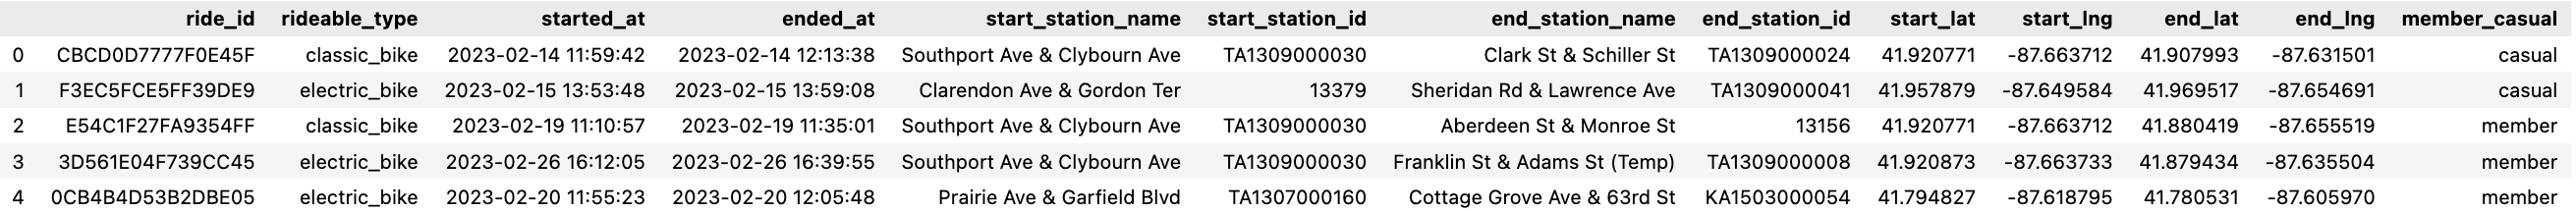
\includegraphics[width=7.2 in, height = 3.3 in]{img1.png}
	\caption{First and last 5 entries of bike rides from the original\_data}
	\label{fig1}
	\end{figure}
	\pagebreak
	
	In Figure \ref{fig1} the multi-index of the DF is shown in the first two columns (month, row\_id). Then looking at the entries themselves we can see that the data consists of 13 columns: 1) ride id, 2) type of bike, 3-4) date and time for the start and end of the ride, 5-12) the name, id, latitude and longitude of the start and end stations, and 13) whether the rider was a casual rider or a member. 
	
	\item \textit{count\_entries}:\\
	The method \textit{count\_entries} is used to find the number of entries within each month, and the average per month. The result is shown in Figure \ref{fig3} left. The dataset contains in total almost 5.7 Million entries, with an average of approximately 480,000 entries per month. From Decemeber to March the number of rides is relatively lower than the average, which is expected as these are cold months. This is confirmed by the peak highlighted in August. After retrieving this information for the original dataset, the duplicates are dropped, and the method is called again. The result of running the method after dropping the duplicates is shown in Figure \ref{fig3} right. The number of entries before and after is identical, therefore the original dataset did not have any duplicates.\\ 
	
	\begin{figure}[h]
	\centering
	\begin{subfigure}{.4\textwidth}
	\hspace{0.5 in}
		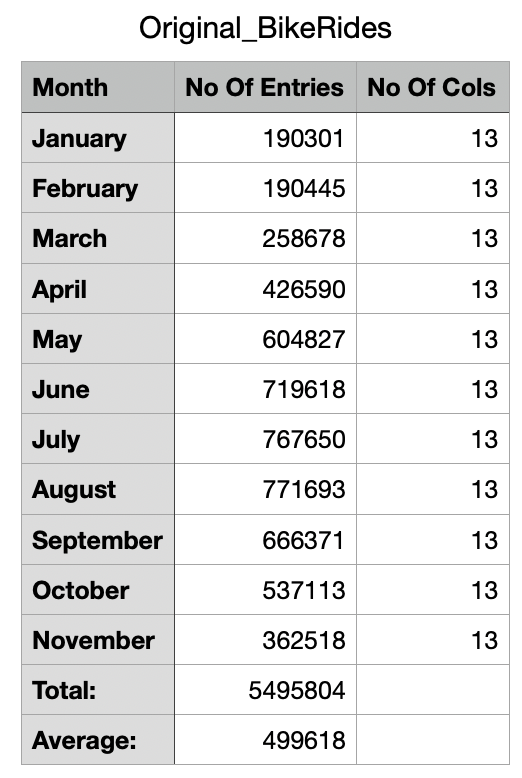
\includegraphics[scale=0.6]{img2.png}
	\end{subfigure}
	\begin{subfigure}{.4\textwidth}
	\hspace{0.5 in}
		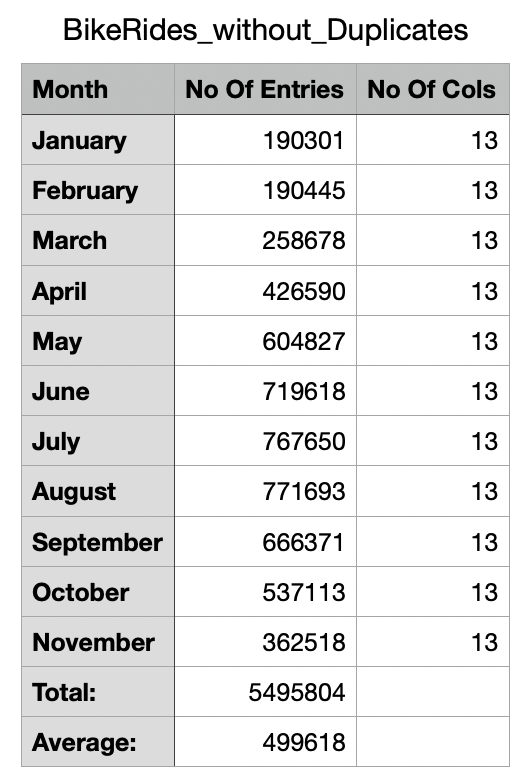
\includegraphics[scale=0.6]{img3.png}
	\end{subfigure}
	\caption{No of entries and average before and after removing duplicates}
	\label{fig3}
	\end{figure}

	\item \textit{get\_null\_percentage}:\\
	This method calculates the percentage of null values for each column and month. The results are shown in Figure \ref{fig4}. As we can see the columns \textit{start\_station\_name}, \textit{start\_station\_id}, \textit{end\_station\_name}, \textit{end\_station\_id} in every month have 13-17\% null values. The columns \textit{end\_lat} and \textit{end\_long} have less than 1\% null values. In order to explore the dataset, as well as these null values a bit further, the number of unique (distinct) values for each column in original\_data[``May"] is calculated and shown in Figure \ref{fig2}. The choice of the month of May is random and should not make a difference. 
	
	\begin{figure}[h]
	\centering
	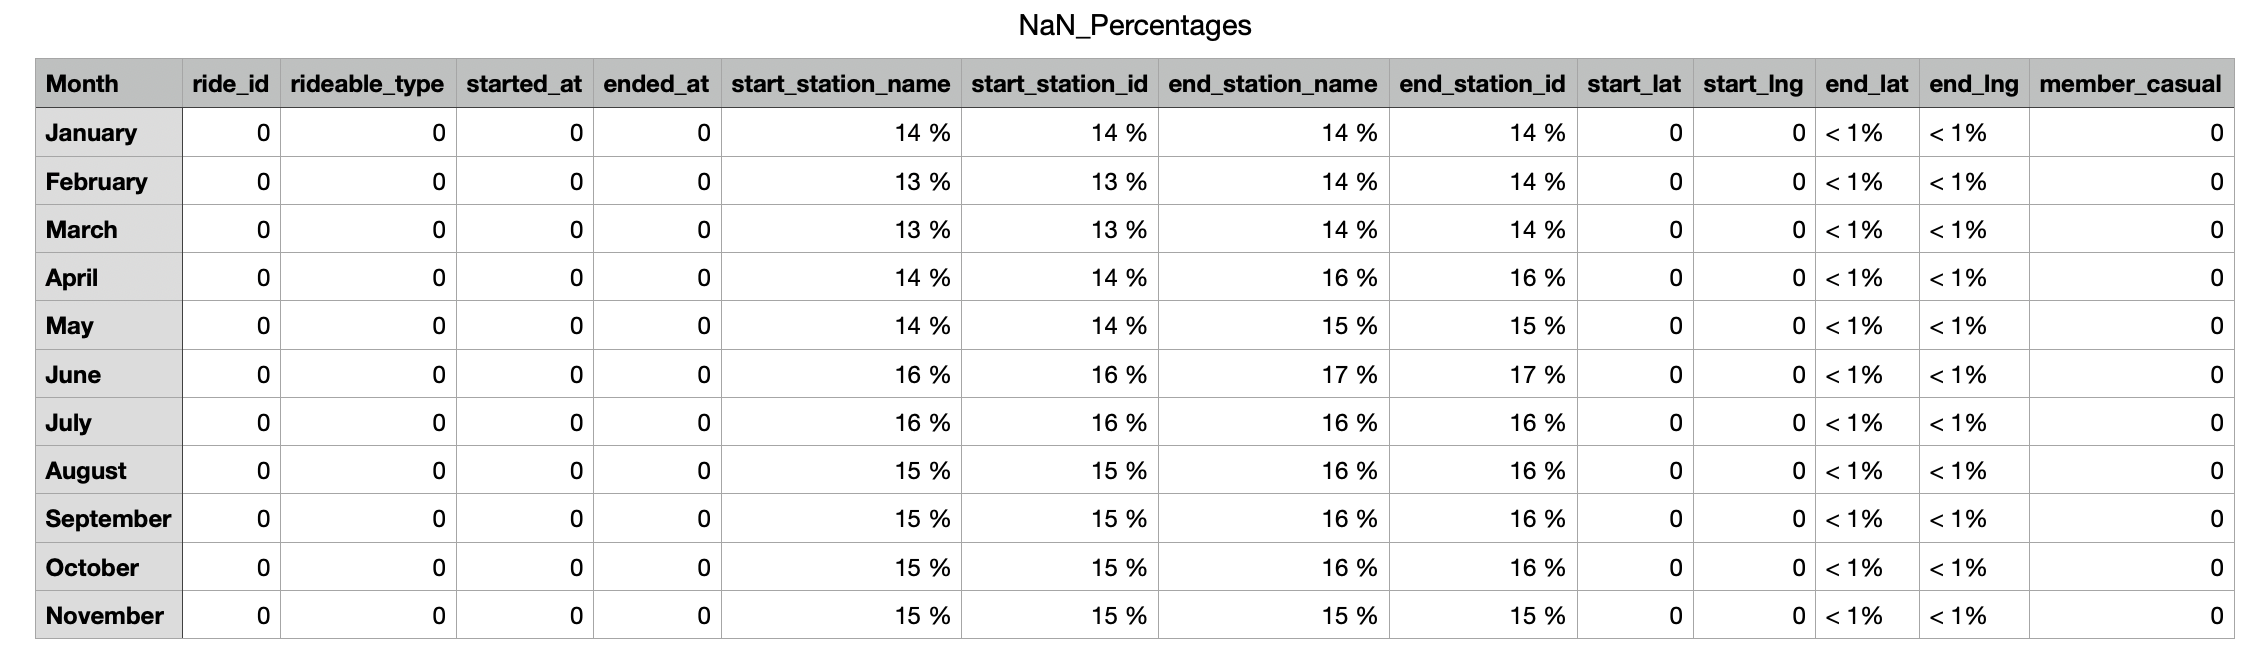
\includegraphics[width=7.2 in, height = 2.5 in]{imgNAN.png}
	\caption{Percentage of null values for each column across the months}
	\label{fig4}
	\end{figure}
	
	\begin{figure}[h]
	\centering
	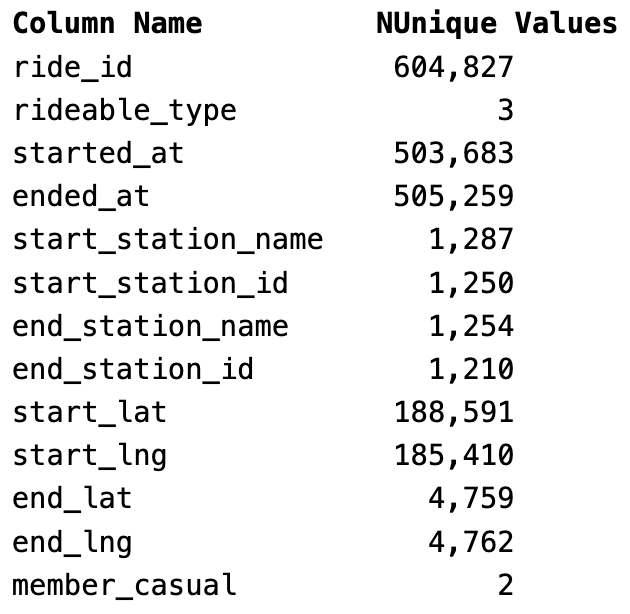
\includegraphics[scale = 0.6]{imgUni.png} %[width=8 in, height = 2 in]
	\caption{No. of unique values for every column in original\_data[``May"]}
	\label{fig2}
	\end{figure}
	
\begin{itemize}
	\item \textit{ride\_id\_unique}  = 604827: as expected, \textit{ride\_id} has as many unique values as the number of entries in the dataframe.
	\item \textit{rideable\_type\_unique} = 3: these 3 unique values are the types of bikes:  [electric\_bike, classic\_bike, docked\_bike].
	\item \textit{started(ended)\_at\_unique} = 503683,  505259: since these are datetimes (yy-mm-dd hh:mm:ss), one may have expected that they would have as many distinct values as the number of entries, since it seems unlikely for more than one rider to have rented a bike at the exact same time down to the second. However, the number of unique values in these columns is less than the number of entries by 17\%. To ensure that these are not duplicate entries but with different \textit{ride\_id}, one of these incidents has been retrieved and is shown in Figure \ref{fig10}. By looking at the values, it is clear that they are indeed different entries but with the exact same start time.
	
	\begin{figure}[h]
	%\centering
	\hspace{0.5cm}
	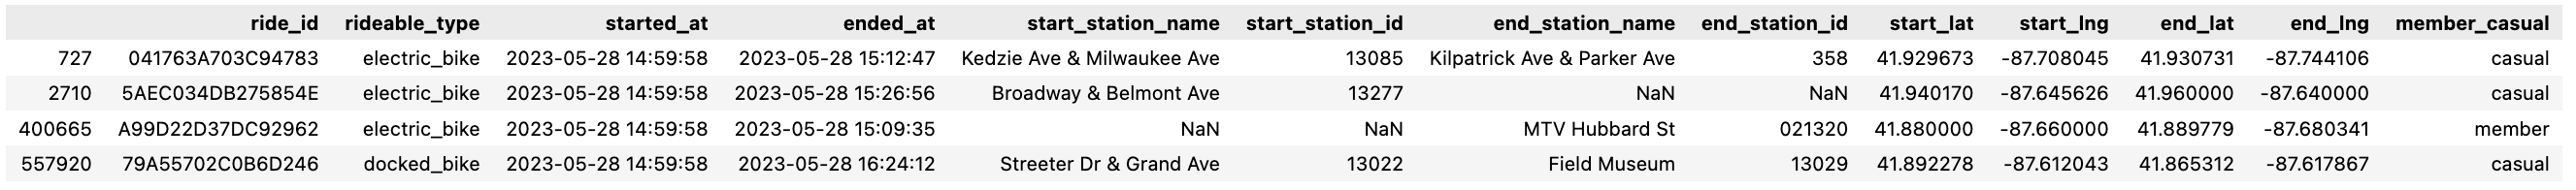
\includegraphics[width=7.2 in, height = 1.3 in]{imgDups1.png}
	\caption{Entries from original\_data[``May"] that have the same \textit{started\_at}}
	\label{fig10}
	\end{figure}
	
	\item \textit{start(end)\_station\_name(id)\_unique} = 1287, 1250, 1254, 1210: since there is a limited number of stations, it is expected that these columns have a smaller number of unique values than the number of entries. However, one would have expected the number of unique station names and station ids to be the same, whereas the ids are less than the names by a small fraction. Which could either by accounted for by the null values or could mean that there are stations that have the different names but the same id.
	\item \textit{start(end)\_lat(long)\_unique} = 188591, 185419, 4759, 4762: the start latitude and longitude numbers seem to be as expected, which is less than the total number of entries, but more than the number of stations (this is based on the assumption that the exact location where a bike is docked can vary within the station especially that the values are given to the $6^{th}$ decimal place). However, there is a large difference between the number of values in the start ($\sim$188000) and the numbers in the end ($\sim$4800) latitude and longitude. This difference cannot be accounted for by the null values in the end columns, since these were less than 1\%. If these values are true, that would mean that users rode there bikes from many start points, but ended up in a much smaller set of points. Which cannot be the case since that would have been reflected in the number of end stations. 
	\item \textit{member\_casual\_unique} = 2: the 2 unique types of riders are: [member, casual].
\end{itemize}
	
	\item \textit{clean\_data}:\\
	After exploring the dataset, we can see that the extractable information can be divided into information about the:
	\begin{enumerate} 
	\item rider (casual/member)
	\item bike (electric/classic/docked)
	\item ride (start-end: time, date, location)
	\end{enumerate}
Since, the goal of the analysis is to find out whether to target converting casual riders into members or not, it seems that all the information is relevant to the analysis, with the exception of the ride location. The geographical location would have been important if for example the goal of the analysis was to find out whether more stations should be added and where to do so. Therefore, since the locations seem to be irrelevant, contain null values and discrepancies, these columns will be dropped. The column \textit{ride\_id} also does not provide any valuable information for the current analysis. Thus, the method \textit{clean\_data1} drops all columns related to geographical location and ride id, which leaves: \textit{rideable\_type}, \textit{started\_at}, \textit{ended\_at}, \textit{member\_casual}. 


Next, is data formatting. We have already looked at the columns \textit{rideable\_type} and \textit{member\_casual}, and ensured that they have the expected values. As for the columns \textit{started\_at} and \textit{ended\_at}, we need to make sure that the \textit{ended\_at} time always comes after \textit{started\_at} time. In order to compare the values, they are first converted in the method \textit{clean\_data1} from strings of characters to a numerical datetime format. Next, by comparing the values and filtering out the cases where the \textit{ended\_at} time is actually before the \textit{started\_at} time, we can see the results in Figure \ref{fig8}.

	\begin{figure}[h]
	\centering
	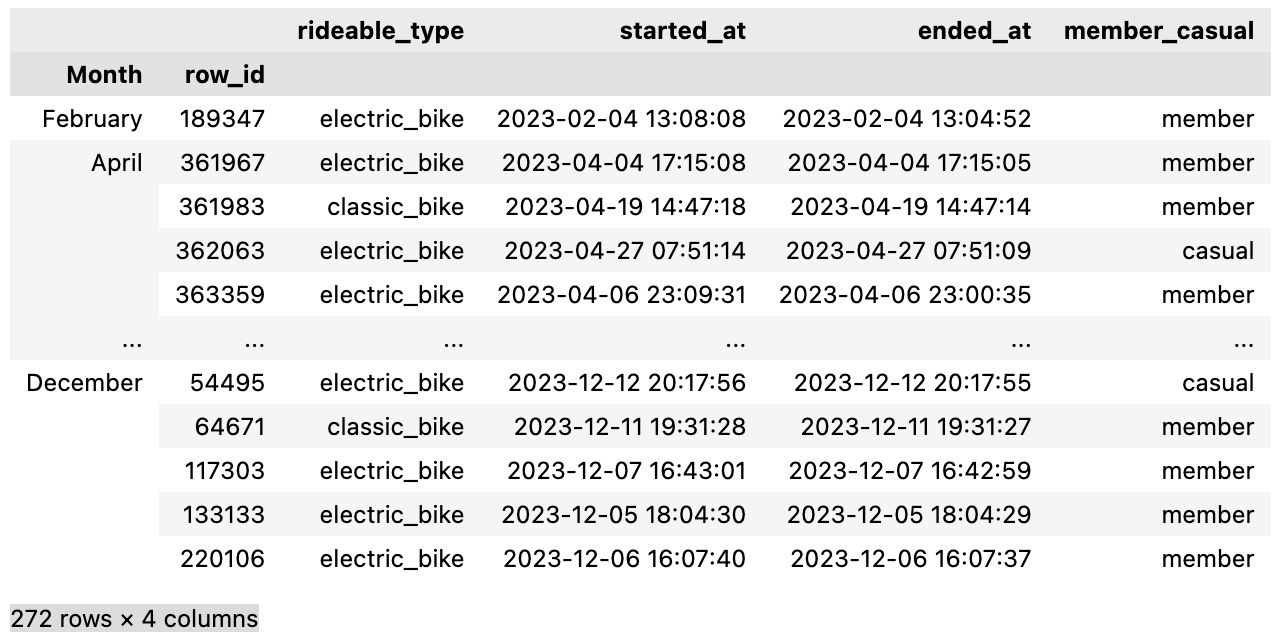
\includegraphics[scale=0.56]{imgNEG.png}
	\caption{Entries where the ended\_at time is before the started\_at time}
	\label{fig8}
	\end{figure}

Looking at the entries in Figure \ref{fig8}, we can see that these are cases when the \textit{ended\_at} time is before the \textit{started\_at} time by just a few seconds. It can be that in these incidents the start and end time were switched due to some glitch, perhaps the bike rental time being only a few seconds (shorter than the server response time). In the entire dataset of approximately 5.5 Million entries, there is a total of 272 entries that have this issue. Since, the dataset is large, we can simply drop these entries.
	
	\end{itemize}

\pagebreak
	
\section*{Analysis:}
\begin{itemize}
\item \textit{prepare\_data}:\\
	The method \textit{prepare\_data} adds two new columns: \textit{ride\_length}: the difference between the columns \textit{ended\_at} and \textit{started\_at} times, and \textit{day\_of\_week}: extracted from the date in \textit{started\_at}. Then the columns \textit{started\_at} and \textit{ended\_at} can be dropped, since they are now redundant.
	
\item \textit{mean\_max\_mode}:\\	
	This method groups the data first by month and then calculates the mean and maximum ride length, as well as the mode of the day of the week; i.e. the day of the week that occurred the most. The method then aggregates the mean, mode and max values across the entire year. The results are shown in Figure \ref{fig9}. The mean ride length varies between 13 - 22 minutes across the months, whereas the maximum ride length is 68 days. 
	
	\begin{figure}[h]
	\centering
	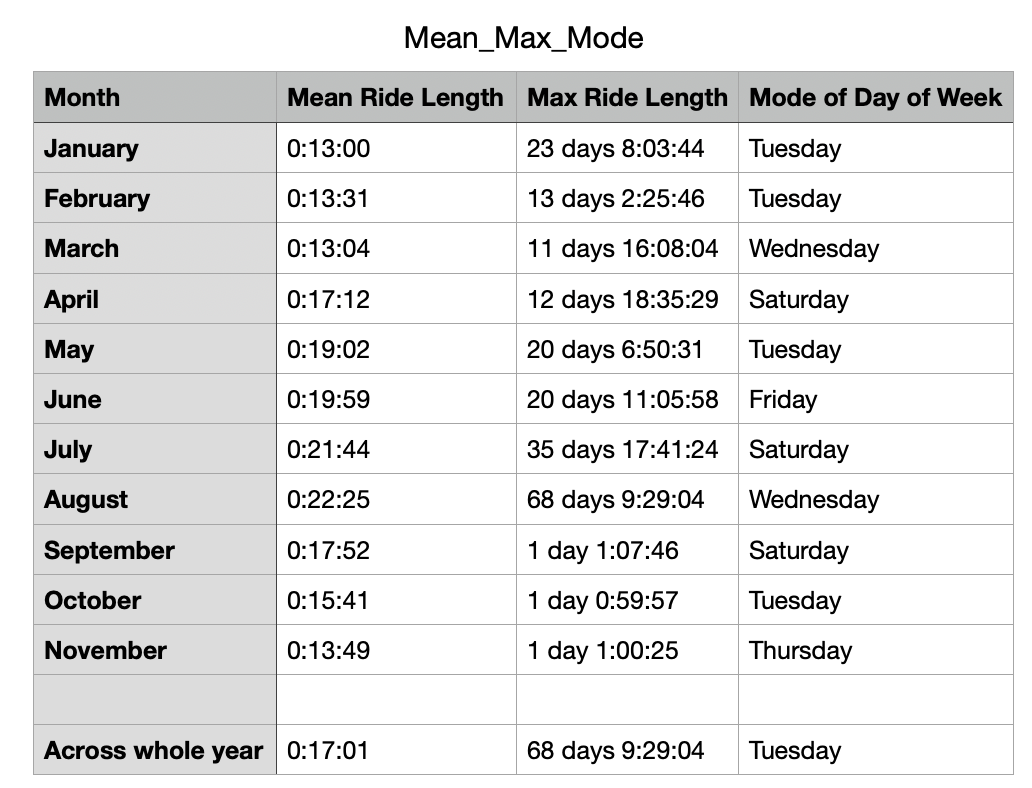
\includegraphics[scale=0.7]{imgMeanMax1.png} 
	\caption{The mean and max ride length, and mode of day of the week}
	\label{fig9}
	\end{figure}
	
	In order to understand how the data shown Figure \ref{fig9} differs between members and casual riders, a pivot table is used to show the maximum and mean value per month by rider type. The table is shown in Figure \ref{fig11}. A quick look shows that the casual riders have longer mean and maximum ride lengths when compared to members. To see this more clearly the mean and maximum ride length are plotted in Figure \ref{fig12}.  
		\pagebreak
		
	\begin{figure}[h]
	\centering
	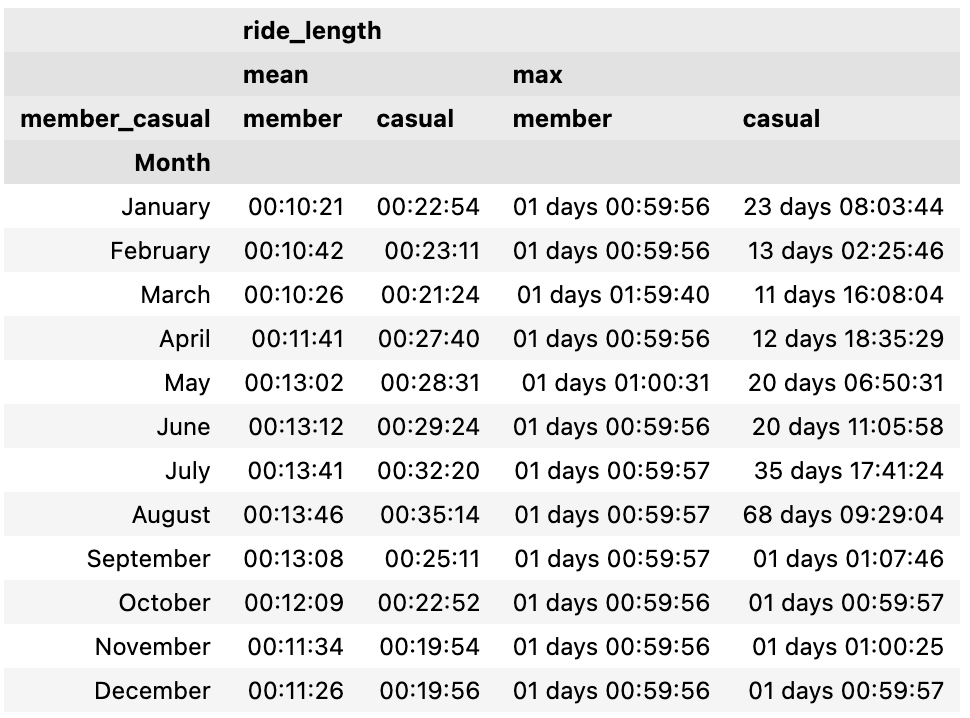
\includegraphics[scale=0.6]{imgMeanMax2.png} 
	\caption{Table of mean and max ride length divided by rider type}
	\label{fig11}
	\end{figure}
	
From the plot of the mean values we observe that casual riders consistently have longer rides, than members across the entire year. Furthermore, the mean ride length for casual riders varies across the year from approximately 20 minutes in the colder months to a peak of 35 minutes in August. In contrast, the mean ride length for members changes only from 10 to 13 minutes. When looking at the maximum ride length plot we can see a similar pattern, where members never have a ride that exceeds one day, whereas casual riders have maximum ride lengths that can go up from 1-68 days. However, it is important to note here that such longer rides, are outliers that occur quite rarely in the dataset. This can be seen when plotting the entire distribution of ride lengths in a box plot shown in Figure \ref{fig13}.  
	
	\begin{figure}[h]
	\centering
	\begin{subfigure}{.45\textwidth}
		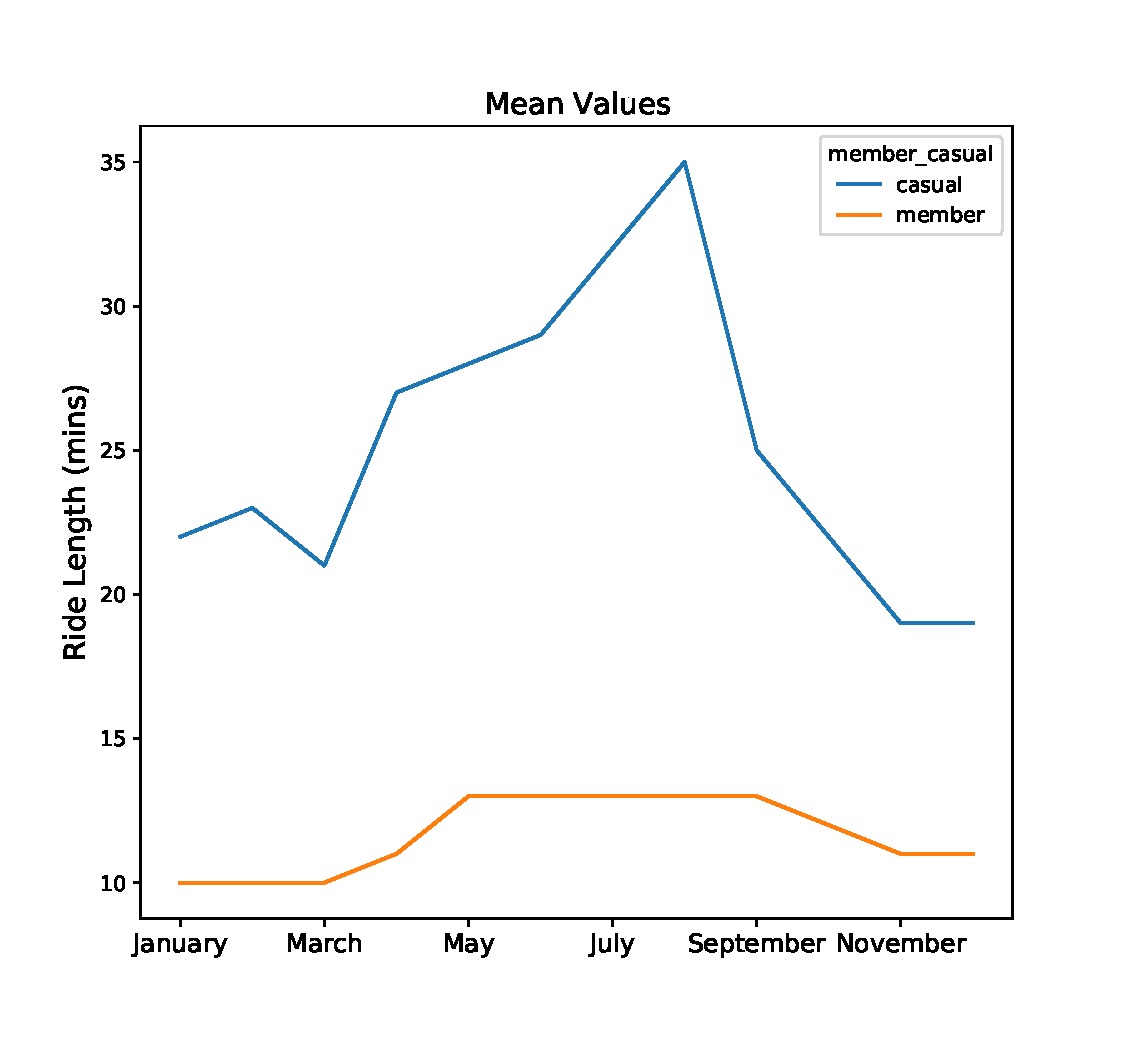
\includegraphics[scale=0.48]{mean_cvsm_month.pdf} 
	\end{subfigure}
	\begin{subfigure}{.4\textwidth}
		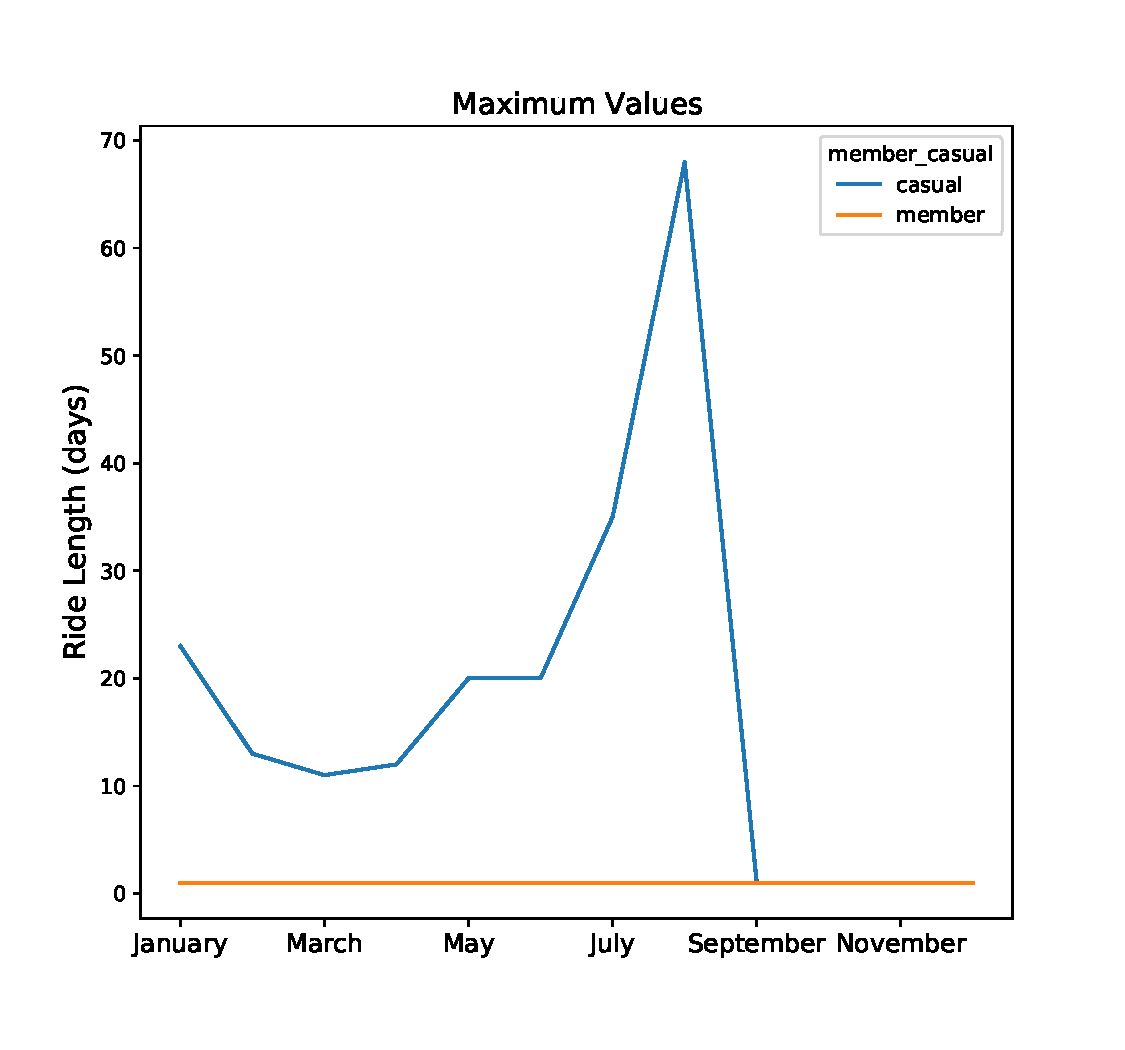
\includegraphics[scale=0.48]{max_cvsm.pdf}
	\end{subfigure}
	\caption{Plots of mean and max ride length divided by rider type grouped by month}
	\label{fig12}
	\end{figure}
	
A box plot typically shows the middle 50\% of the distribution inside a box, then the lower and upper 25\% are shown by the whiskers, and finally circles represent outliers. We can see that the entire distribution of ride lengths for casual rider is between 0-50 minutes, with outliers in the range from 1-70 days. As for members, the ride lengths vary between 0-30 minutes, with outliers in the range 1- 25 hours. Therefore, if we ignore the outliers, the difference between the ride lengths for casual riders and members can be seen side by side in Figure \ref{fig15}.
	
	\begin{figure}[h]
	\hspace{-0.5in}
	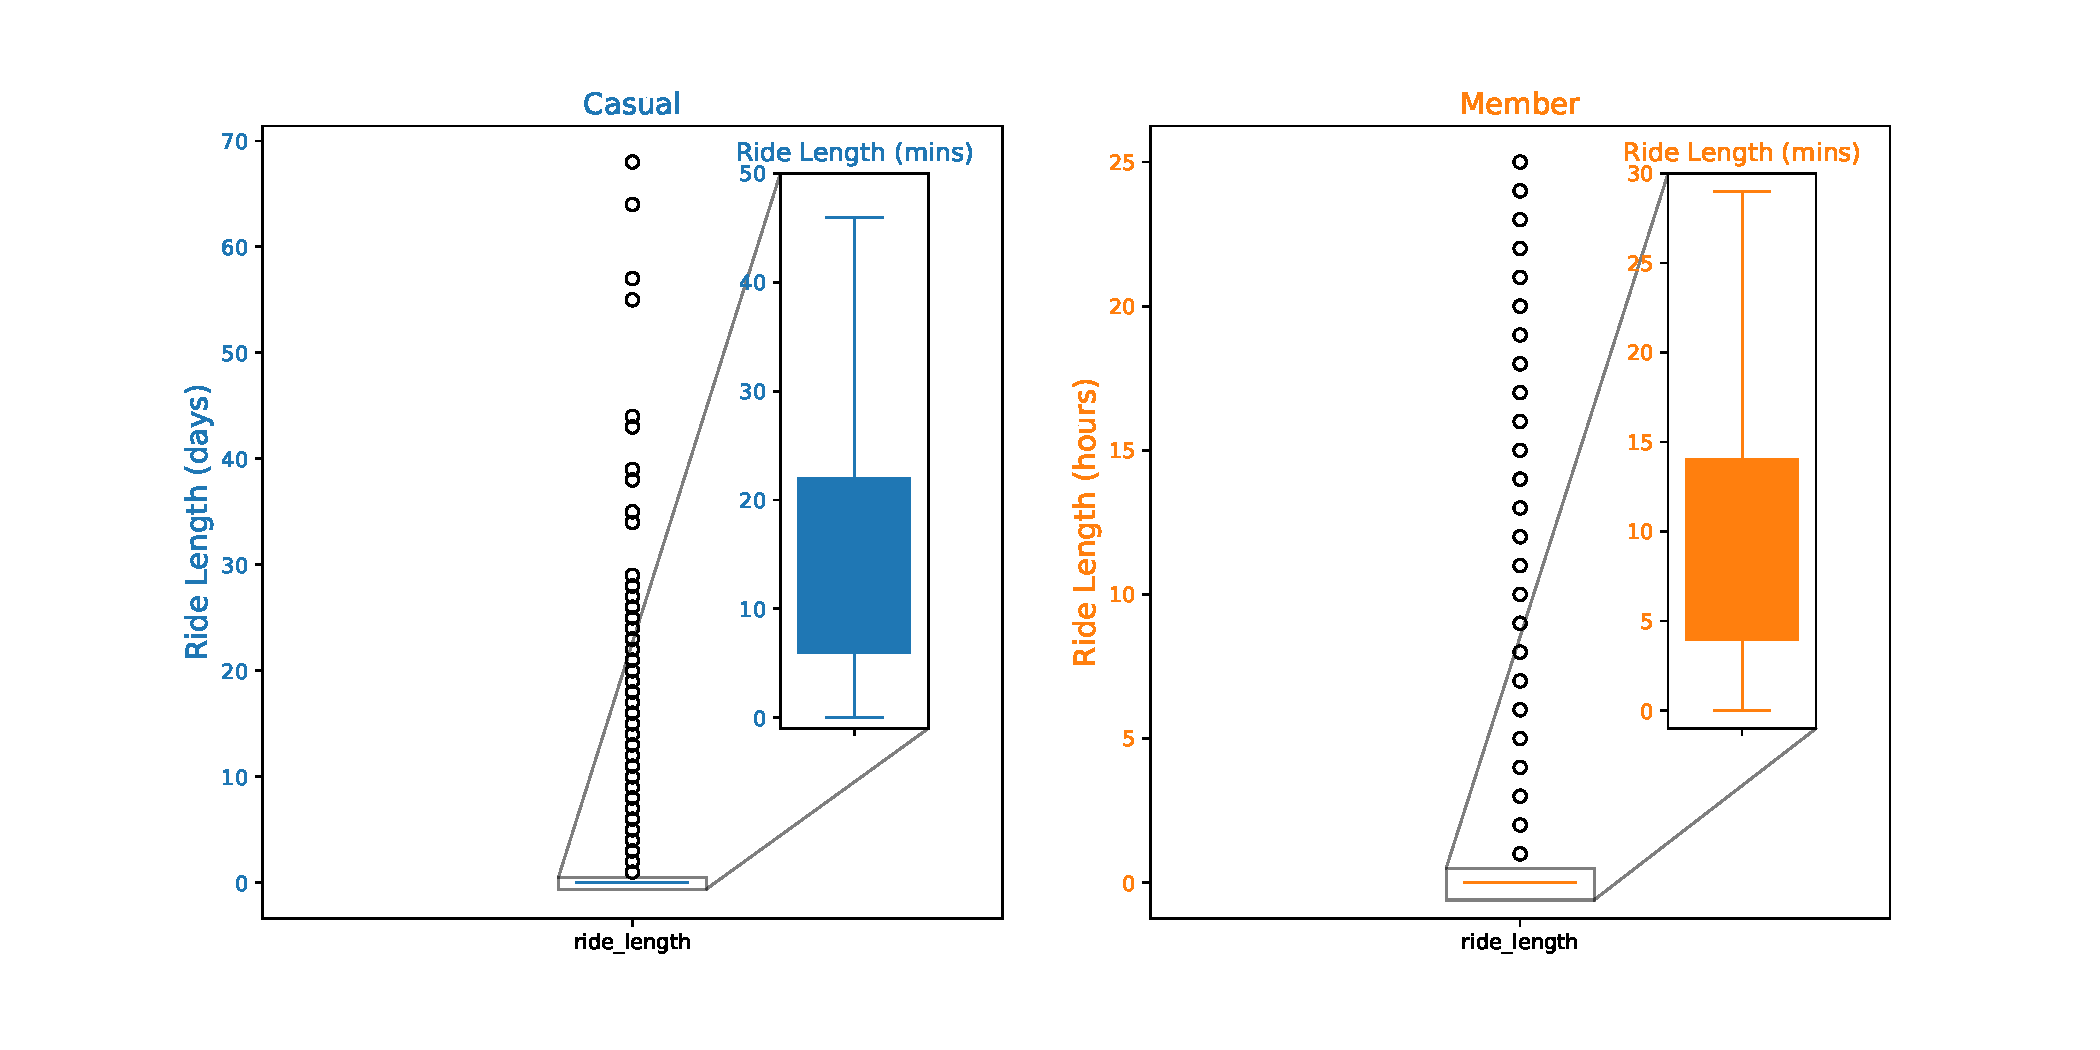
\includegraphics[scale=0.6]{boxplot_distribution.pdf} 
	\caption{Box plots of the ride length distributions. Left: casual riders, Right: members}
	\label{fig13}
	\end{figure}
	
	\begin{figure}[h]
	\centering
	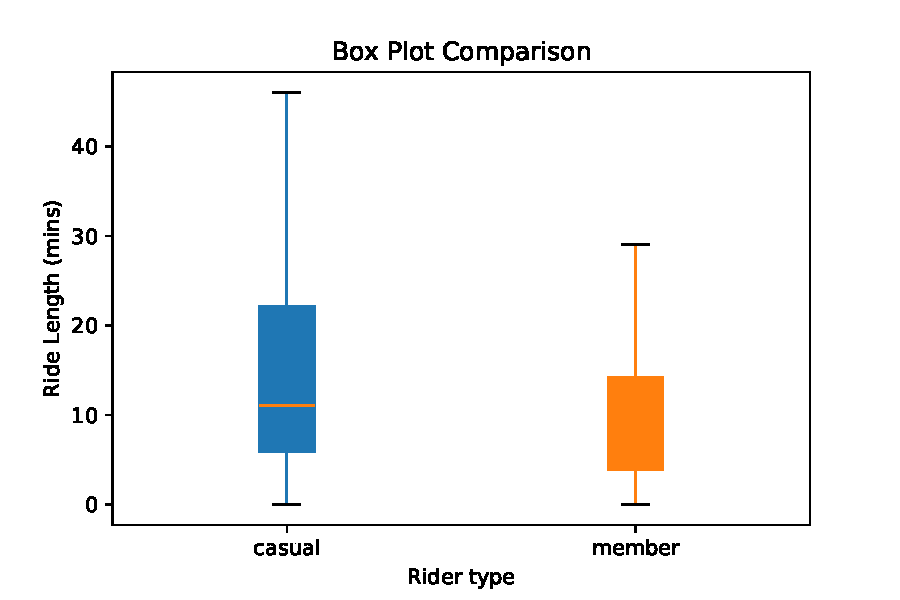
\includegraphics[scale=0.6]{boxplot_distribution2.pdf} 
	\caption{Box plot comparison of the ride length distributions casual and member riders}
	\label{fig15}
	\end{figure}

In order to determine how significant this difference is we need to look at the number rides for the different rider types. 
	
So far we have been looking at the data by first grouping it using the month. In order to get a different perspective, we now look at the mean value of the ride length, however when the data is grouped using the day of the week. The result can be seen in Figure \ref{fig14}. Here we see the same higher average for the casual riders when compared to the members.  

	\begin{figure}[h]
	\centering
	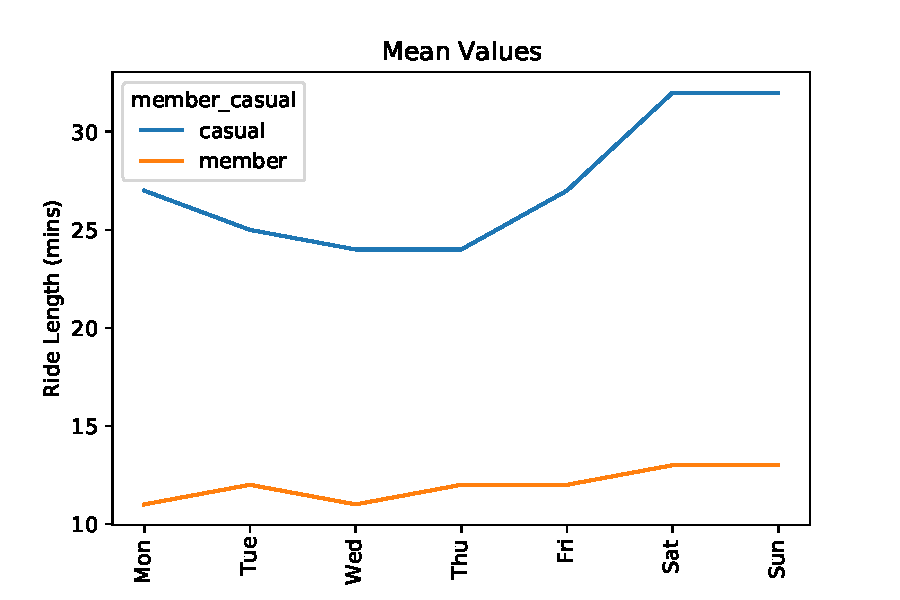
\includegraphics[scale=0.6]{mean_cvsm_dayofweek.pdf} 
	\caption{Plot of mean ride length divided by rider type grouped by day of the week}
	\label{fig14}
	\end{figure}
	
\end{itemize}

\section*{Conclusion:}

In general, casual riders always have a longer rides. And the behaviour across seasons or days varies with a peak in August and the weekends. We can see that the entire distribution of ride lengths for casual rider is between 0-50 minutes, with outliers in the range from 1-70 days. As for members, the ride lengths vary between 0-30 minutes, with outliers in the range 1- 25 hours. Therefore, if we ignore the outliers, the casual riders have a higher ride length by 66\%.

\end{document}